% Options for packages loaded elsewhere
\PassOptionsToPackage{unicode}{hyperref}
\PassOptionsToPackage{hyphens}{url}
\PassOptionsToPackage{dvipsnames,svgnames,x11names}{xcolor}
%
\documentclass[
  ignorenonframetext,
]{beamer}
\usepackage{pgfpages}
\setbeamertemplate{caption}[numbered]
\setbeamertemplate{caption label separator}{: }
\setbeamercolor{caption name}{fg=normal text.fg}
\beamertemplatenavigationsymbolsempty
% Prevent slide breaks in the middle of a paragraph
\widowpenalties 1 10000
\raggedbottom

\usepackage{amsmath,amssymb}
\usepackage{iftex}
\ifPDFTeX
  \usepackage[T1]{fontenc}
  \usepackage[utf8]{inputenc}
  \usepackage{textcomp} % provide euro and other symbols
\else % if luatex or xetex
  \usepackage{unicode-math}
  \defaultfontfeatures{Scale=MatchLowercase}
  \defaultfontfeatures[\rmfamily]{Ligatures=TeX,Scale=1}
\fi
\usepackage{lmodern}
\usetheme[]{AnnArbor}
\usecolortheme{dolphin}
\usefonttheme{structurebold}
\ifPDFTeX\else  
    % xetex/luatex font selection
\fi
% Use upquote if available, for straight quotes in verbatim environments
\IfFileExists{upquote.sty}{\usepackage{upquote}}{}
\IfFileExists{microtype.sty}{% use microtype if available
  \usepackage[]{microtype}
  \UseMicrotypeSet[protrusion]{basicmath} % disable protrusion for tt fonts
}{}
\makeatletter
\@ifundefined{KOMAClassName}{% if non-KOMA class
  \IfFileExists{parskip.sty}{%
    \usepackage{parskip}
  }{% else
    \setlength{\parindent}{0pt}
    \setlength{\parskip}{6pt plus 2pt minus 1pt}}
}{% if KOMA class
  \KOMAoptions{parskip=half}}
\makeatother
\usepackage{xcolor}
\newif\ifbibliography
\setlength{\emergencystretch}{3em} % prevent overfull lines
\setcounter{secnumdepth}{-\maxdimen} % remove section numbering


\providecommand{\tightlist}{%
  \setlength{\itemsep}{0pt}\setlength{\parskip}{0pt}}\usepackage{longtable,booktabs,array}
\usepackage{calc} % for calculating minipage widths
\usepackage{caption}
% Make caption package work with longtable
\makeatletter
\def\fnum@table{\tablename~\thetable}
\makeatother
\usepackage{graphicx}
\makeatletter
\def\maxwidth{\ifdim\Gin@nat@width>\linewidth\linewidth\else\Gin@nat@width\fi}
\def\maxheight{\ifdim\Gin@nat@height>\textheight\textheight\else\Gin@nat@height\fi}
\makeatother
% Scale images if necessary, so that they will not overflow the page
% margins by default, and it is still possible to overwrite the defaults
% using explicit options in \includegraphics[width, height, ...]{}
\setkeys{Gin}{width=\maxwidth,height=\maxheight,keepaspectratio}
% Set default figure placement to htbp
\makeatletter
\def\fps@figure{htbp}
\makeatother
% definitions for citeproc citations
\NewDocumentCommand\citeproctext{}{}
\NewDocumentCommand\citeproc{mm}{%
  \begingroup\def\citeproctext{#2}\cite{#1}\endgroup}
\makeatletter
 % allow citations to break across lines
 \let\@cite@ofmt\@firstofone
 % avoid brackets around text for \cite:
 \def\@biblabel#1{}
 \def\@cite#1#2{{#1\if@tempswa , #2\fi}}
\makeatother
\newlength{\cslhangindent}
\setlength{\cslhangindent}{1.5em}
\newlength{\csllabelwidth}
\setlength{\csllabelwidth}{3em}
\newenvironment{CSLReferences}[2] % #1 hanging-indent, #2 entry-spacing
 {\begin{list}{}{%
  \setlength{\itemindent}{0pt}
  \setlength{\leftmargin}{0pt}
  \setlength{\parsep}{0pt}
  % turn on hanging indent if param 1 is 1
  \ifodd #1
   \setlength{\leftmargin}{\cslhangindent}
   \setlength{\itemindent}{-1\cslhangindent}
  \fi
  % set entry spacing
  \setlength{\itemsep}{#2\baselineskip}}}
 {\end{list}}
\usepackage{calc}
\newcommand{\CSLBlock}[1]{\hfill\break\parbox[t]{\linewidth}{\strut\ignorespaces#1\strut}}
\newcommand{\CSLLeftMargin}[1]{\parbox[t]{\csllabelwidth}{\strut#1\strut}}
\newcommand{\CSLRightInline}[1]{\parbox[t]{\linewidth - \csllabelwidth}{\strut#1\strut}}
\newcommand{\CSLIndent}[1]{\hspace{\cslhangindent}#1}

\usepackage{booktabs}
\usepackage{longtable}
\usepackage{array}
\usepackage{multirow}
\usepackage{wrapfig}
\usepackage{float}
\usepackage{colortbl}
\usepackage{pdflscape}
\usepackage{tabu}
\usepackage{threeparttable}
\usepackage{threeparttablex}
\usepackage[normalem]{ulem}
\usepackage{makecell}
\usepackage{xcolor}

% logo
\titlegraphic{
\includegraphics[width=4cm]{000_images/logo-blue-vertical}}
\logo{\ifnum\thepage>1
\includegraphics[width=0.5cm]{000_images/logo-blue-vertical}\fi}

% UMNG: Manual de image institucional

% Colors

% Umng
\definecolor{yellow}{HTML}{fdc600}
\definecolor{red-dark}{HTML}{841e35}

% Estudios a Distancia
\definecolor{blue1}{HTML}{12245b}
\definecolor{blue2}{HTML}{767ca6}
\definecolor{blue3}{HTML}{cad2ec}

% Modify items
\setbeamercolor{palette primary}{bg=blue3}
\setbeamercolor{palette tertiary}{bg=blue1}
\setbeamercolor{frametitle}{bg=yellow}

% Hyperlinks
\hypersetup{
  linkcolor=red-dark,
  citecolor=red-dark
}

\makeatletter
\@ifpackageloaded{caption}{}{\usepackage{caption}}
\AtBeginDocument{%
\ifdefined\contentsname
  \renewcommand*\contentsname{Table of contents}
\else
  \newcommand\contentsname{Table of contents}
\fi
\ifdefined\listfigurename
  \renewcommand*\listfigurename{List of Figures}
\else
  \newcommand\listfigurename{List of Figures}
\fi
\ifdefined\listtablename
  \renewcommand*\listtablename{List of Tables}
\else
  \newcommand\listtablename{List of Tables}
\fi
\ifdefined\figurename
  \renewcommand*\figurename{Figure}
\else
  \newcommand\figurename{Figure}
\fi
\ifdefined\tablename
  \renewcommand*\tablename{Table}
\else
  \newcommand\tablename{Table}
\fi
}
\@ifpackageloaded{float}{}{\usepackage{float}}
\floatstyle{ruled}
\@ifundefined{c@chapter}{\newfloat{codelisting}{h}{lop}}{\newfloat{codelisting}{h}{lop}[chapter]}
\floatname{codelisting}{Listing}
\newcommand*\listoflistings{\listof{codelisting}{List of Listings}}
\makeatother
\makeatletter
\makeatother
\makeatletter
\@ifpackageloaded{caption}{}{\usepackage{caption}}
\@ifpackageloaded{subcaption}{}{\usepackage{subcaption}}
\makeatother

\ifLuaTeX
\usepackage[bidi=basic]{babel}
\else
\usepackage[bidi=default]{babel}
\fi
\babelprovide[main,import]{english}
% get rid of language-specific shorthands (see #6817):
\let\LanguageShortHands\languageshorthands
\def\languageshorthands#1{}
\ifLuaTeX
  \usepackage{selnolig}  % disable illegal ligatures
\fi
\usepackage{bookmark}

\IfFileExists{xurl.sty}{\usepackage{xurl}}{} % add URL line breaks if available
\urlstyle{same} % disable monospaced font for URLs
\hypersetup{
  pdftitle={Introduction},
  pdfauthor={Luis Francisco Gómez López},
  pdflang={en},
  colorlinks=true,
  linkcolor={Maroon},
  filecolor={Maroon},
  citecolor={Blue},
  urlcolor={Blue},
  pdfcreator={LaTeX via pandoc}}


\title{Introduction}
\author{Luis Francisco Gómez López}
\date{2024-07-13}
\institute{FAEDIS}

\begin{document}
\frame{\titlepage}

\renewcommand*\contentsname{Table of contents}
\begin{frame}[allowframebreaks]
  \frametitle{Table of contents}
  \tableofcontents[hideallsubsections]
\end{frame}

\section{Please Read Me}\label{please-read-me}

\begin{frame}{}
\phantomsection\label{section}
\begin{itemize}
\item
  Check the message \textbf{Welcome greeting} published in the News
  Bulletin Board.
\item
  Dear student please edit your profile uploading a photo where your
  face is clearly visible.
\item
  The purpose of the virtual meetings is to answer questions and not to
  make a summary of the study material.
\item
  This presentation is based on
  (\citeproc{ref-cardenas_introduccion_2020}{Cardenas 2020, chap. 1})
\end{itemize}
\end{frame}

\section{Purpose}\label{purpose}

\begin{frame}{}
\phantomsection\label{section-1}
Identify the main characteristics of the Colombian economy, especially
those that differentiate it from other economies
\end{frame}

\section{Economic environment and the
Company}\label{economic-environment-and-the-company}

\begin{frame}{}
\phantomsection\label{section-2}
\begin{figure}

\centering{

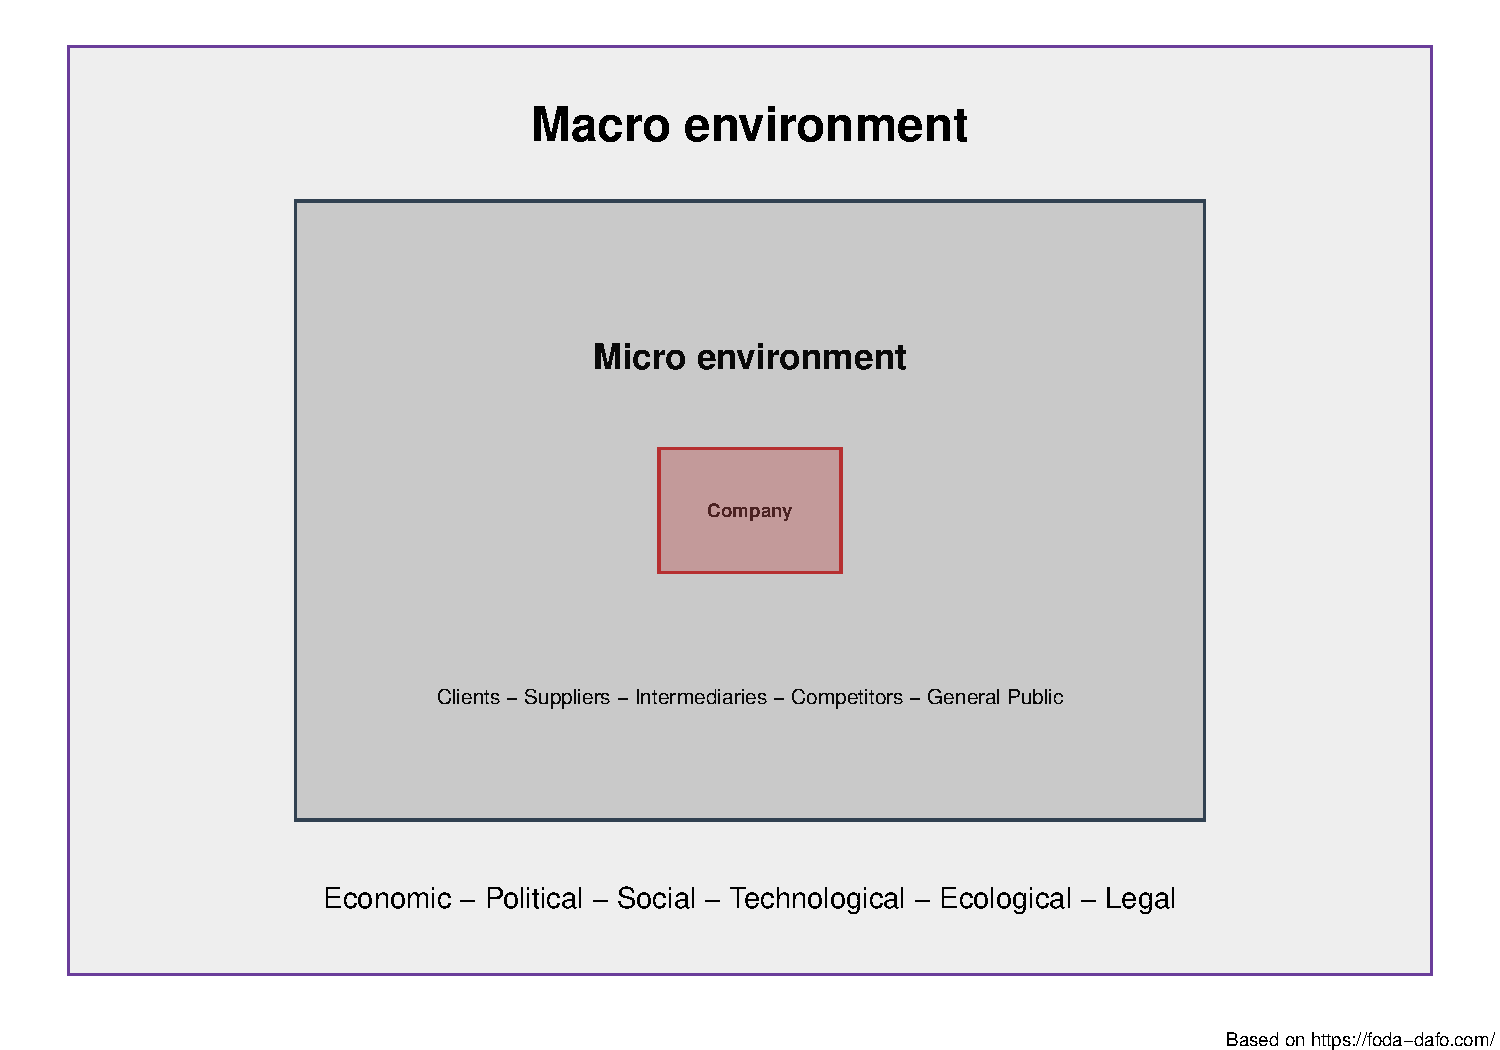
\includegraphics[width=0.85\textwidth,height=\textheight]{001_intro_files/figure-beamer/fig-econ-env-macro-1.pdf}

}

\caption{\label{fig-econ-env-macro}Set of economic factors and forces
that influence the development of an organization}

\end{figure}%
\end{frame}

\section{Population}\label{population}

\begin{frame}{}
\phantomsection\label{section-3}
\begin{figure}

\centering{

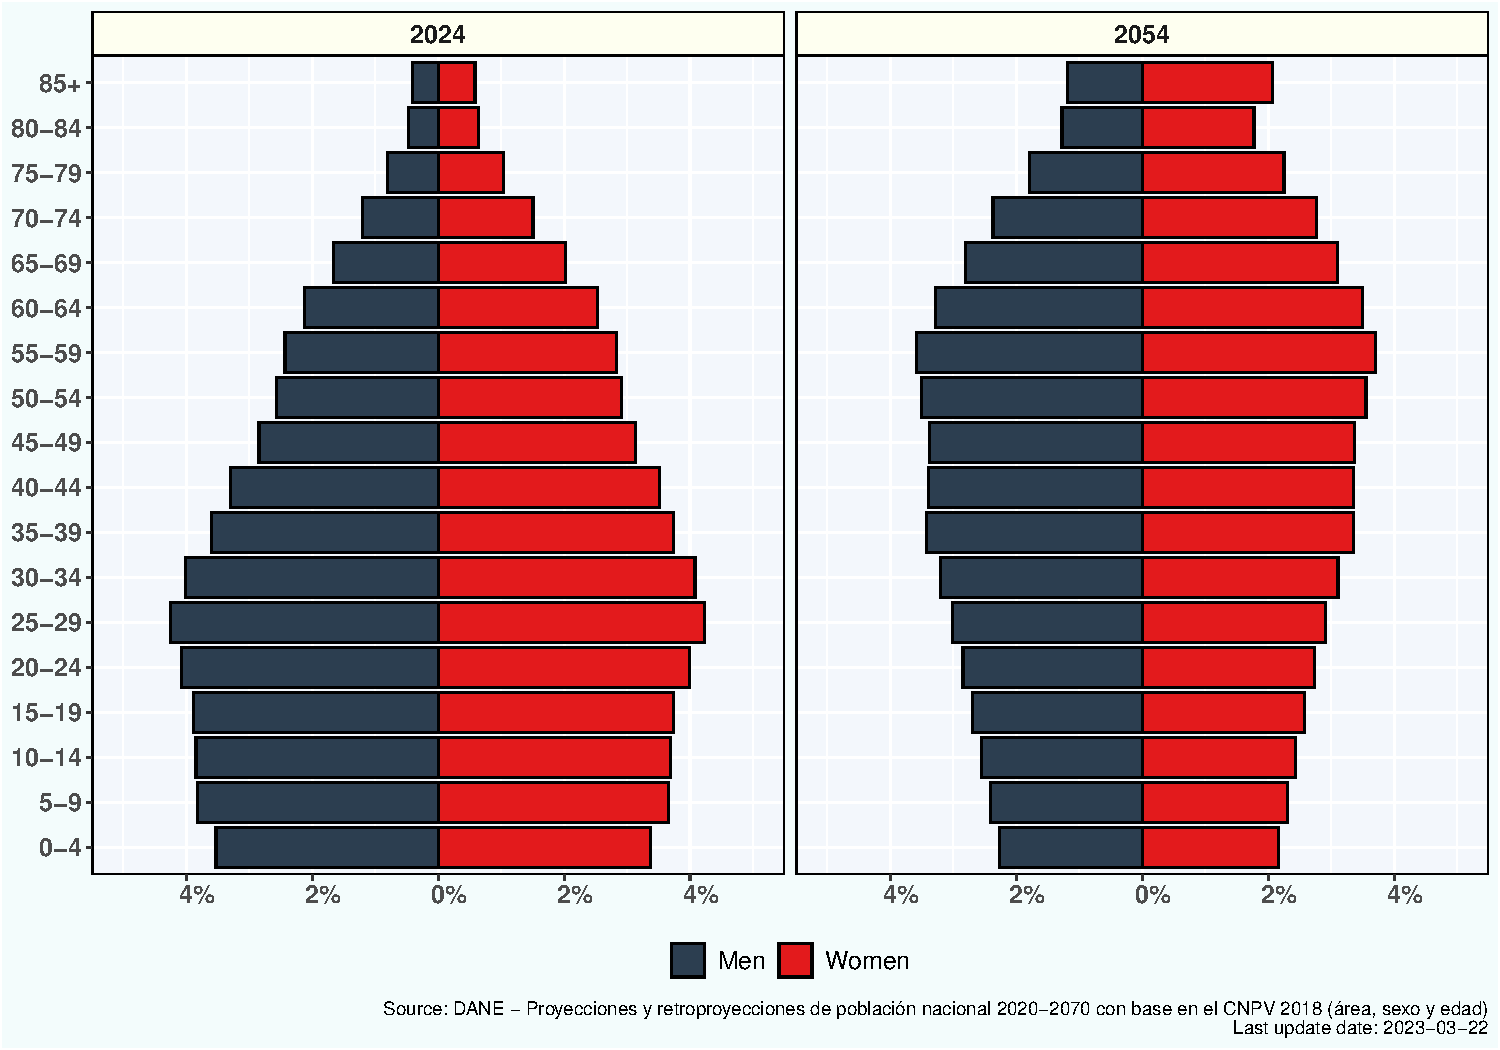
\includegraphics[width=0.85\textwidth,height=\textheight]{001_intro_files/figure-beamer/fig-population-col-1.pdf}

}

\caption{\label{fig-population-col}Population pyramid in Colombia}

\end{figure}%
\end{frame}

\section{Mean height}\label{mean-height}

\begin{frame}{}
\phantomsection\label{section-4}
\begin{figure}

\centering{

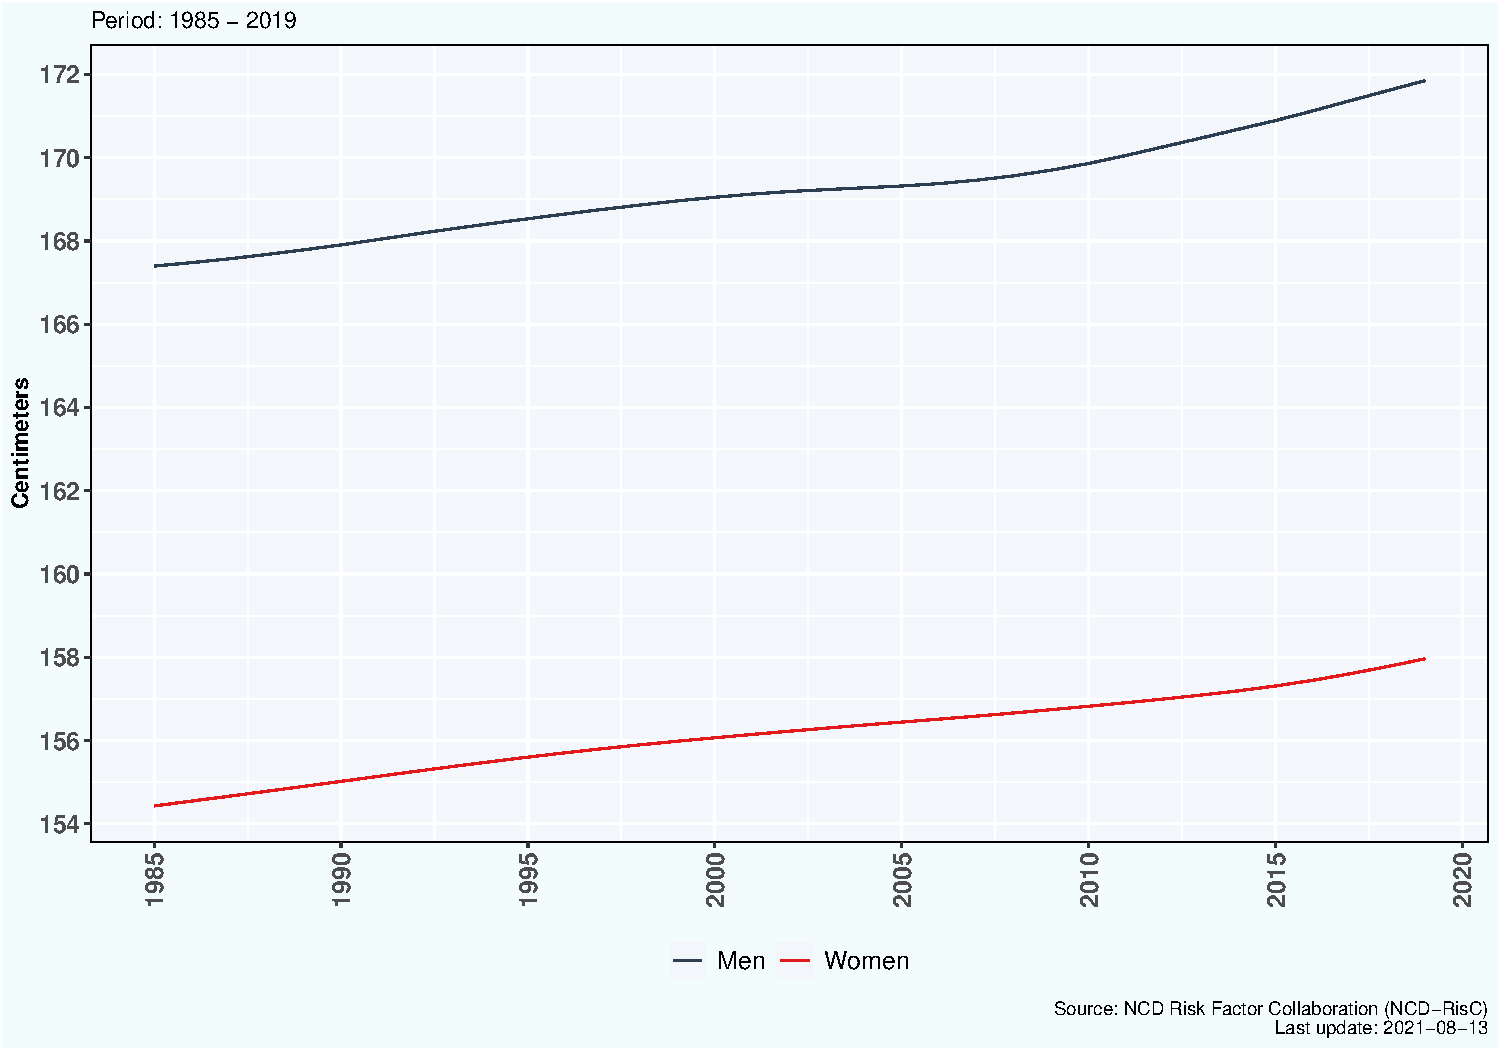
\includegraphics[width=0.85\textwidth,height=\textheight]{001_intro_files/figure-beamer/fig-avg-height-19-year-old-col-1.pdf}

}

\caption{\label{fig-avg-height-19-year-old-col}Average height by gender
for 19 year olds in Colombia}

\end{figure}%
\end{frame}

\section{Household income}\label{household-income}

\begin{frame}{}
\phantomsection\label{section-5}
\begin{itemize}
\item
  \textbf{ingtotug}: \emph{``Ingreso total de la unidad de gasto
  \textbf{antes} de imputación de arriendo a propietarios y
  usufructuarios''} (\citeproc{ref-dnp_pobreza_2012}{DNP and DANE 2012,
  16--17})

  \begin{itemize}
  \tightlist
  \item
    \emph{Ingreso monetario primera actividad (IMPA)}
  \item
    \emph{Ingreso en especie (IE)}
  \item
    \emph{Ingreso segunda actividad (ISA)}
  \item
    \emph{Ingreso monetario de desocupados e inactivos (IMDI)}
  \item
    \emph{Ingresos por otras fuentes (IOF)}
  \end{itemize}
\item
  \textbf{ingtotugarr}: ``Ingreso total de la unidad de gasto con
  imputación de arriendo a propietarios y usufructuarios''
  (\citeproc{ref-dnp_pobreza_2012}{DNP and DANE 2012, 24--26})

  \begin{itemize}
  \tightlist
  \item
    Modulo B Datos de la Vivienda: 11. Si tuviera que pagar arriendo por
    esta vivienda, ¿cuánto estima que tendría que pagar mensualmente?
    (\citeproc{ref-dane_cuestionario_2019}{DANE 2019}, p 2)
  \end{itemize}
\end{itemize}
\end{frame}

\begin{frame}{}
\phantomsection\label{section-6}
\begin{figure}

\centering{

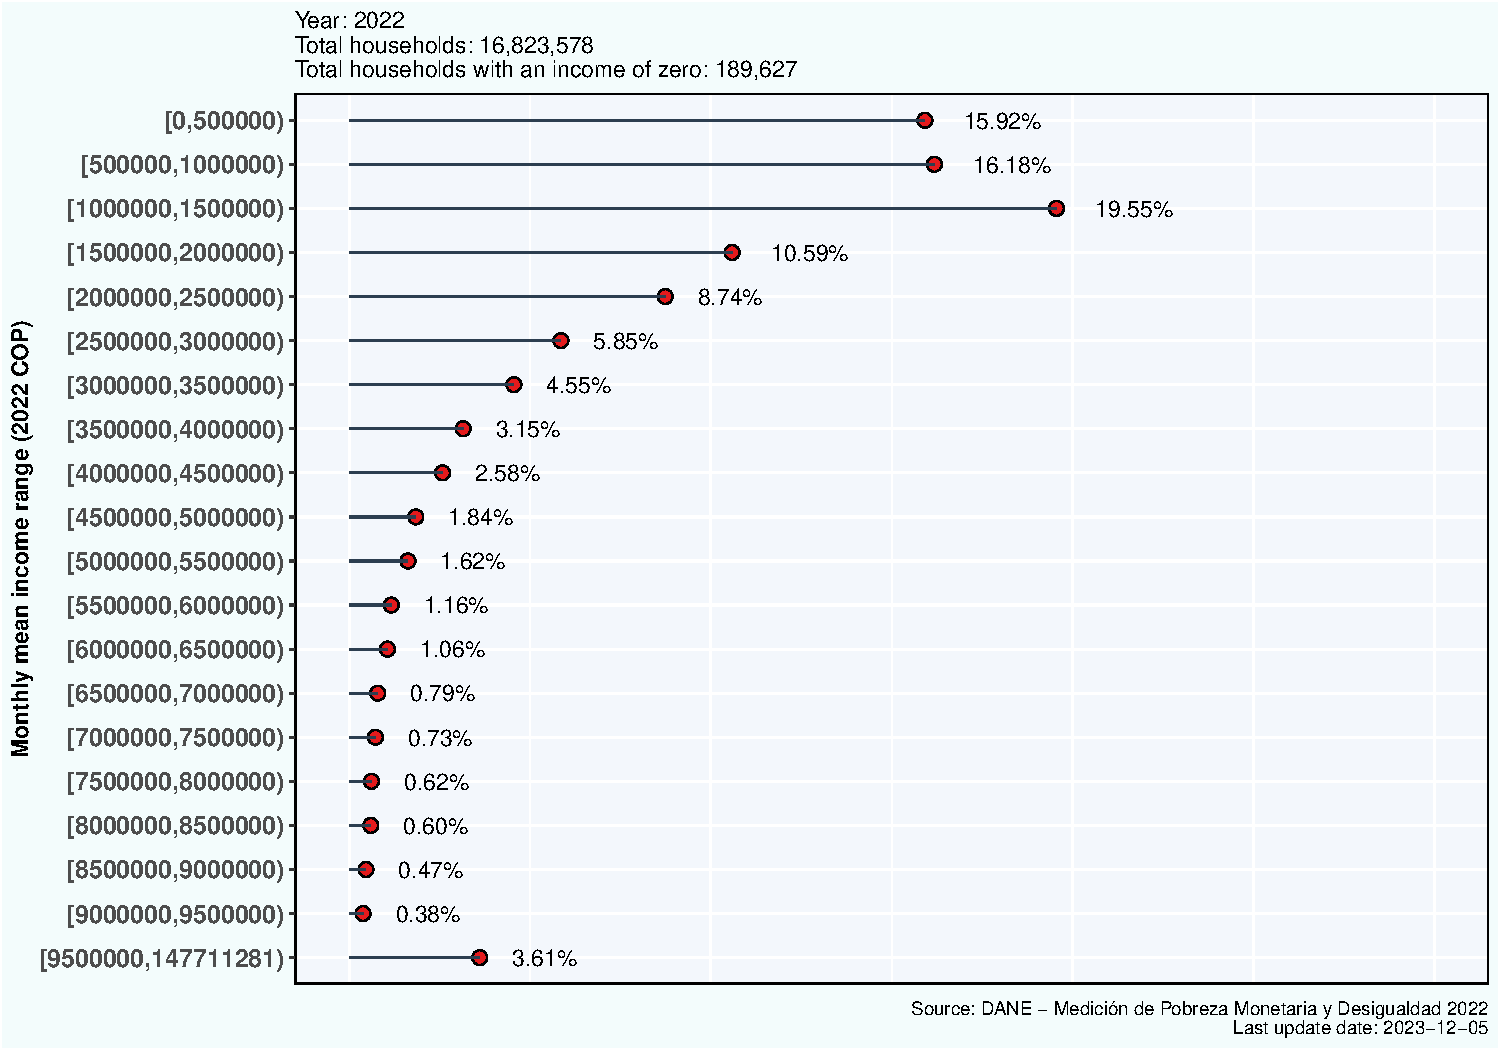
\includegraphics[width=0.85\textwidth,height=\textheight]{001_intro_files/figure-beamer/fig-household-income-col-1.pdf}

}

\caption{\label{fig-household-income-col}Household income distribution
in Colombia}

\end{figure}%
\end{frame}

\begin{frame}{}
\phantomsection\label{section-7}
\begin{itemize}
\item
  If you want to explore more about this topic using data from the year
  2019 check out\footnote<.->{Observatorio Fiscal de la Pontifica
    Universidad Javeriana}:

  \begin{itemize}
  \item
    \url{https://www.ofiscal.org/} \textgreater{} Interactúa
    \textgreater{} Calcule dónde se ubica su hogar según su ingreso →

    \begin{itemize}
    \tightlist
    \item
      \url{https://www.ofiscal.org/ingresosxhogares}
    \end{itemize}
  \end{itemize}
\item
  If you want to explore more about this topic from around the world in
  a visual way check out\footnote<.->{Dollar Street}:

  \begin{itemize}
  \item
    \href{https://youtu.be/u4L130DkdOw}{See how the rest of the world
    lives, organized by income} (Configure spanish subtitles in the
    setting options)
  \item
    \url{https://www.gapminder.org} \textgreater{} Resources
    \textgreater{} Tools \textgreater{} Dollar Street

    \begin{itemize}
    \tightlist
    \item
      \url{https://www.gapminder.org/dollar-street}
    \end{itemize}
  \end{itemize}
\end{itemize}
\end{frame}

\section{Individuals per household}\label{individuals-per-household}

\begin{frame}{}
\phantomsection\label{section-8}
\begin{figure}

\centering{

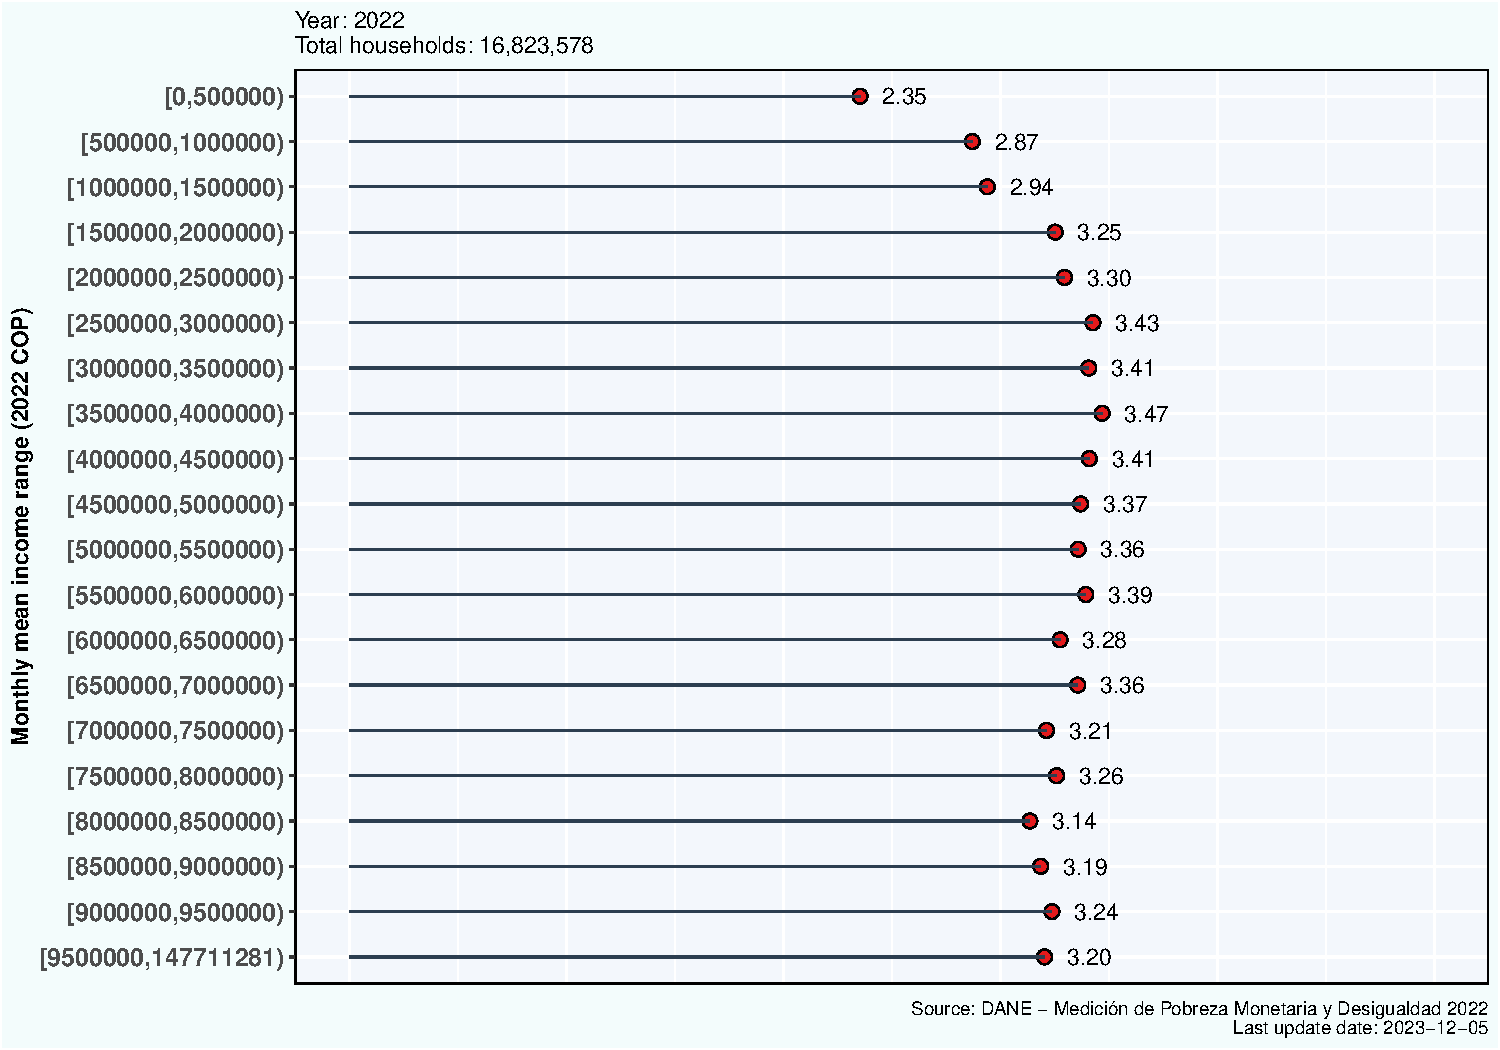
\includegraphics[width=0.85\textwidth,height=\textheight]{001_intro_files/figure-beamer/fig-household-size-col-1.pdf}

}

\caption{\label{fig-household-size-col}Mean individuals per household by
income range in Colombia}

\end{figure}%
\end{frame}

\section{Housing ownership}\label{housing-ownership}

\begin{frame}{}
\phantomsection\label{section-9}
\begin{itemize}
\item
  Housing (vivienda) ownership status\footnote<.->{For a detail
    definition of these categories checkout
    (\citeproc{ref-dane_manual_2022}{DANE 2022b, 35})}

  \begin{itemize}
  \tightlist
  \item
    \emph{Propia, totalmente pagada}
  \item
    \emph{Propia, la están pagando}
  \item
    \emph{En arriendo o subarriendo}
  \item
    \emph{En usufructo}
  \item
    \emph{Posesión sin título}
  \item
    \emph{Propiedad colectiva}
  \item
    \emph{Otra}
  \end{itemize}
\item
  The concept of housing (vivienda) is different from a household
  (hogar)

  \begin{itemize}
  \tightlist
  \item
    Zero or more households can live in a housing (vivienda)
  \item
    For a detail definition of a househould check out
    (\citeproc{ref-united_nations_principles_2017}{United Nations 2017,
    38, 2.33})
  \end{itemize}
\end{itemize}
\end{frame}

\begin{frame}{}
\phantomsection\label{section-10}
\begin{figure}

\centering{

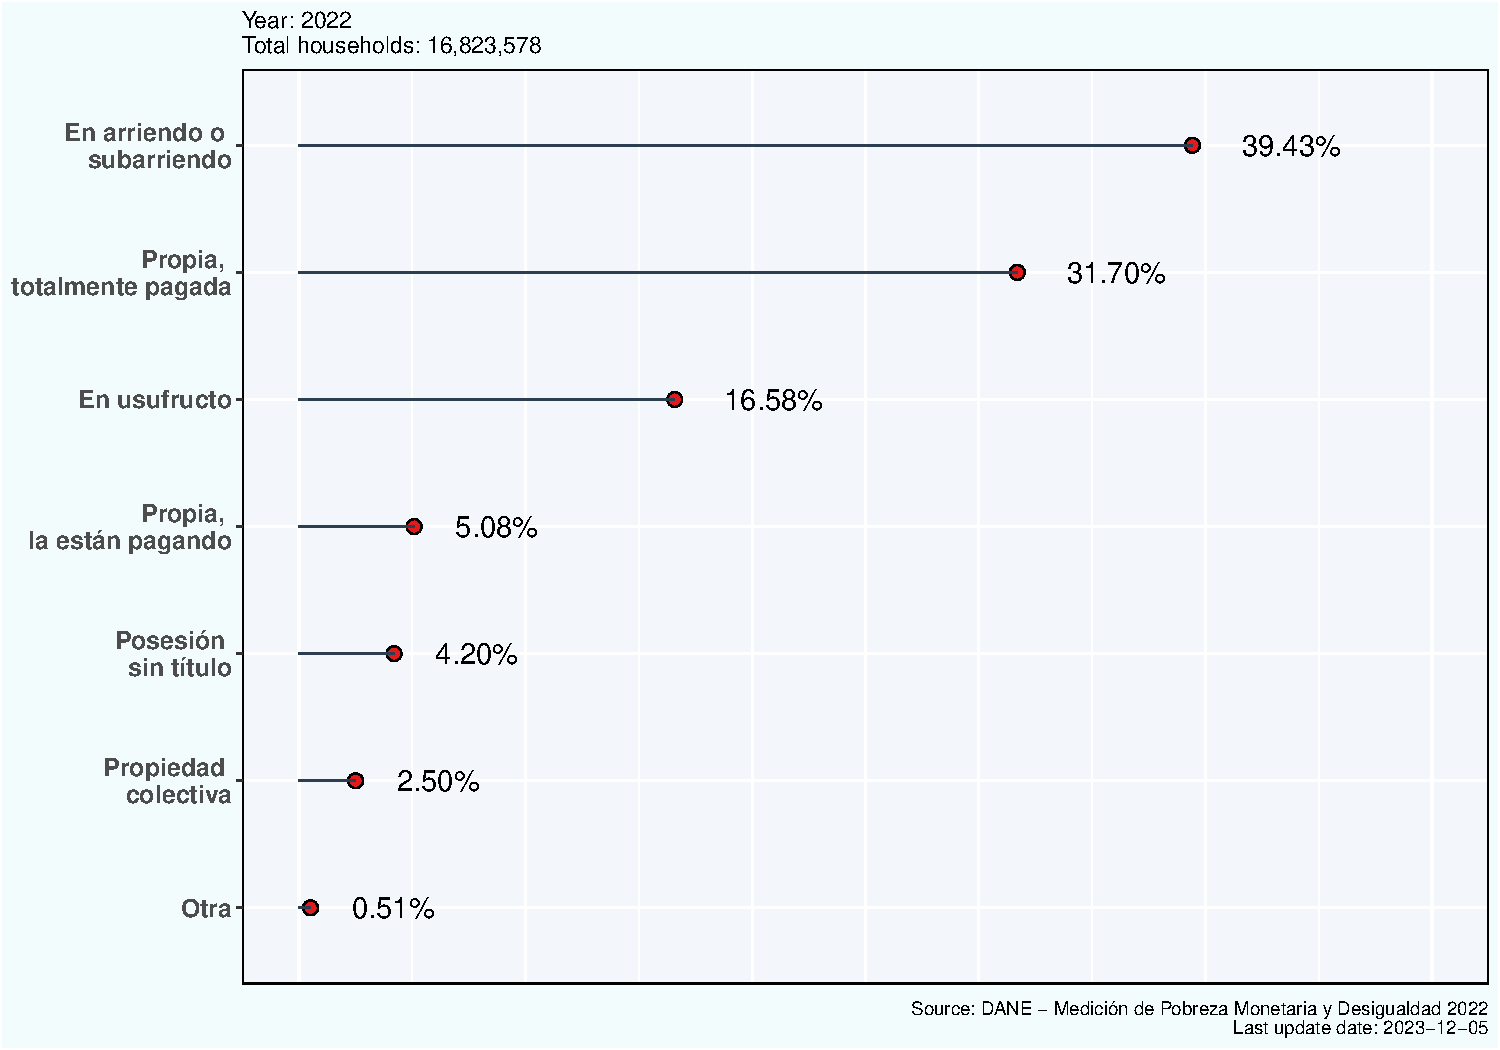
\includegraphics[width=0.85\textwidth,height=\textheight]{001_intro_files/figure-beamer/fig-housing-ownership-col-1.pdf}

}

\caption{\label{fig-housing-ownership-col}Housing ownership status of
households in Colombia}

\end{figure}%
\end{frame}

\section{School education system and
bilingualism}\label{school-education-system-and-bilingualism}

\begin{frame}{}
\phantomsection\label{section-11}
\begin{figure}

\centering{

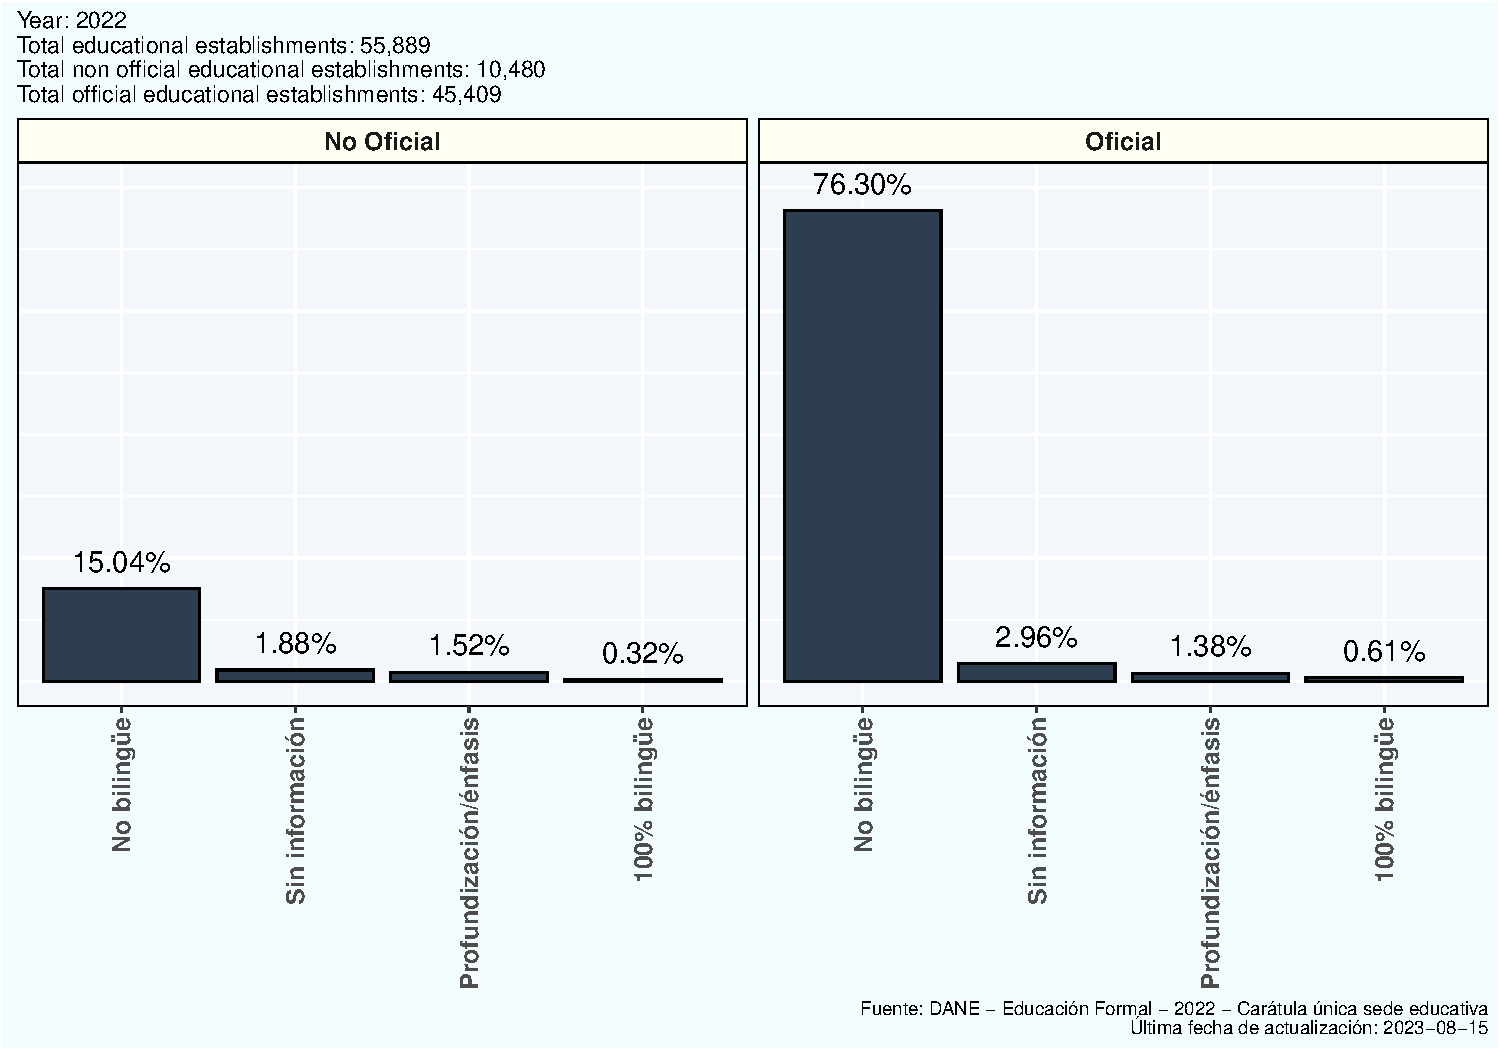
\includegraphics[width=0.85\textwidth,height=\textheight]{001_intro_files/figure-beamer/fig-bilingualism-school-col-1.pdf}

}

\caption{\label{fig-bilingualism-school-col}Bilingualism and educational
establishments (preschool, elementary, middle and high school) in
Colombia}

\end{figure}%
\end{frame}

\section{Aggregate value}\label{aggregate-value}

\begin{frame}{}
\phantomsection\label{section-12}
\begin{table}

\caption{\label{tbl-isic-col-1}ISIC adapted for Colombia
(\citeproc{ref-dane_clasificacion_2022}{DANE 2022a, 134--677})}

\centering{

\centering\begingroup\fontsize{9}{11}\selectfont

\begin{tabular}{>{\raggedright\arraybackslash}p{0.3in}>{\raggedright\arraybackslash}p{0.3in}>{\raggedright\arraybackslash}p{3.4in}}
\toprule
\textbf{Section} & \textbf{Division} & \textbf{Description}\\
\midrule
\cellcolor{gray!10}{A} & \cellcolor{gray!10}{01-03} & \cellcolor{gray!10}{Agricultura, ganadería, caza, silvicultura y pesca}\\
B & 05-09 & Explotación de minas y canteras\\
\cellcolor{gray!10}{C} & \cellcolor{gray!10}{10-33} & \cellcolor{gray!10}{Industrias manufactureras}\\
D & 35 & Suministro de electricidad, gas, vapor, y aire acondicionado\\
E & 36-39 & Distribución de agua; evacuación y tratamiento de aguas residuales, gestión de desechos y
\cellcolor{gray!10}{actividades de saneamiento ambiental}\\
\addlinespace
F & 41-43 & Construcción\\
\cellcolor{gray!10}{G} & \cellcolor{gray!10}{45-47} & \cellcolor{gray!10}{Comercio al por mayor y al por menor; reparación de vehículos automotores y motocicletas}\\
H & 49-53 & Transporte y almacenamiento\\
\cellcolor{gray!10}{I} & \cellcolor{gray!10}{55-56} & \cellcolor{gray!10}{Alojamiento y servicios de comida}\\
J & 58-63 & Información y comunicaciones\\
\addlinespace
\cellcolor{gray!10}{K} & \cellcolor{gray!10}{64-66} & \cellcolor{gray!10}{Actividades financieras y de seguros}\\
\bottomrule
\end{tabular}
\endgroup{}

}

\end{table}%
\end{frame}

\begin{frame}{}
\phantomsection\label{section-13}
\begin{table}

\caption{\label{tbl-isic-col-2}ISIC adapted for Colombia
(\citeproc{ref-dane_clasificacion_2022}{DANE 2022a, 134--677})}

\centering{

\centering\begingroup\fontsize{9}{11}\selectfont

\begin{tabular}{>{\raggedright\arraybackslash}p{0.3in}>{\raggedright\arraybackslash}p{0.3in}>{\raggedright\arraybackslash}p{3.4in}}
\toprule
\textbf{Section} & \textbf{Division} & \textbf{Description}\\
\midrule
\cellcolor{gray!10}{L} & \cellcolor{gray!10}{68} & \cellcolor{gray!10}{Actividades inmobiliarias}\\
M & 69-75 & Actividades profesionales, científicas y técnicas\\
\cellcolor{gray!10}{N} & \cellcolor{gray!10}{77-82} & \cellcolor{gray!10}{Actividades de servicios administrativos y de poyo}\\
O & 84 & Administración pública y defensa; planes de seguridad social de afiliación obligatoria\\
\cellcolor{gray!10}{P} & \cellcolor{gray!10}{85} & \cellcolor{gray!10}{Educación}\\
\addlinespace
Q & 86-88 & Actividades de atención de la salud humana y de asistencia social\\
\cellcolor{gray!10}{R} & \cellcolor{gray!10}{90-93} & \cellcolor{gray!10}{Actividades artísticas, de entretenimiento y recreación}\\
S & 94-96 & Otras actividades de servicios\\
T & 97-98 & Actividades de los hogares en calidad de empleadores; actividades no diferenciadas de los
\cellcolor{gray!10}{hogares individuales como productores de bienes y servicios para uso propio}\\
U & 99 & Actividades de organizaciones y entidades extraterritoriales\\
\bottomrule
\end{tabular}
\endgroup{}

}

\end{table}%
\end{frame}

\begin{frame}{}
\phantomsection\label{section-14}
\begin{figure}

\centering{

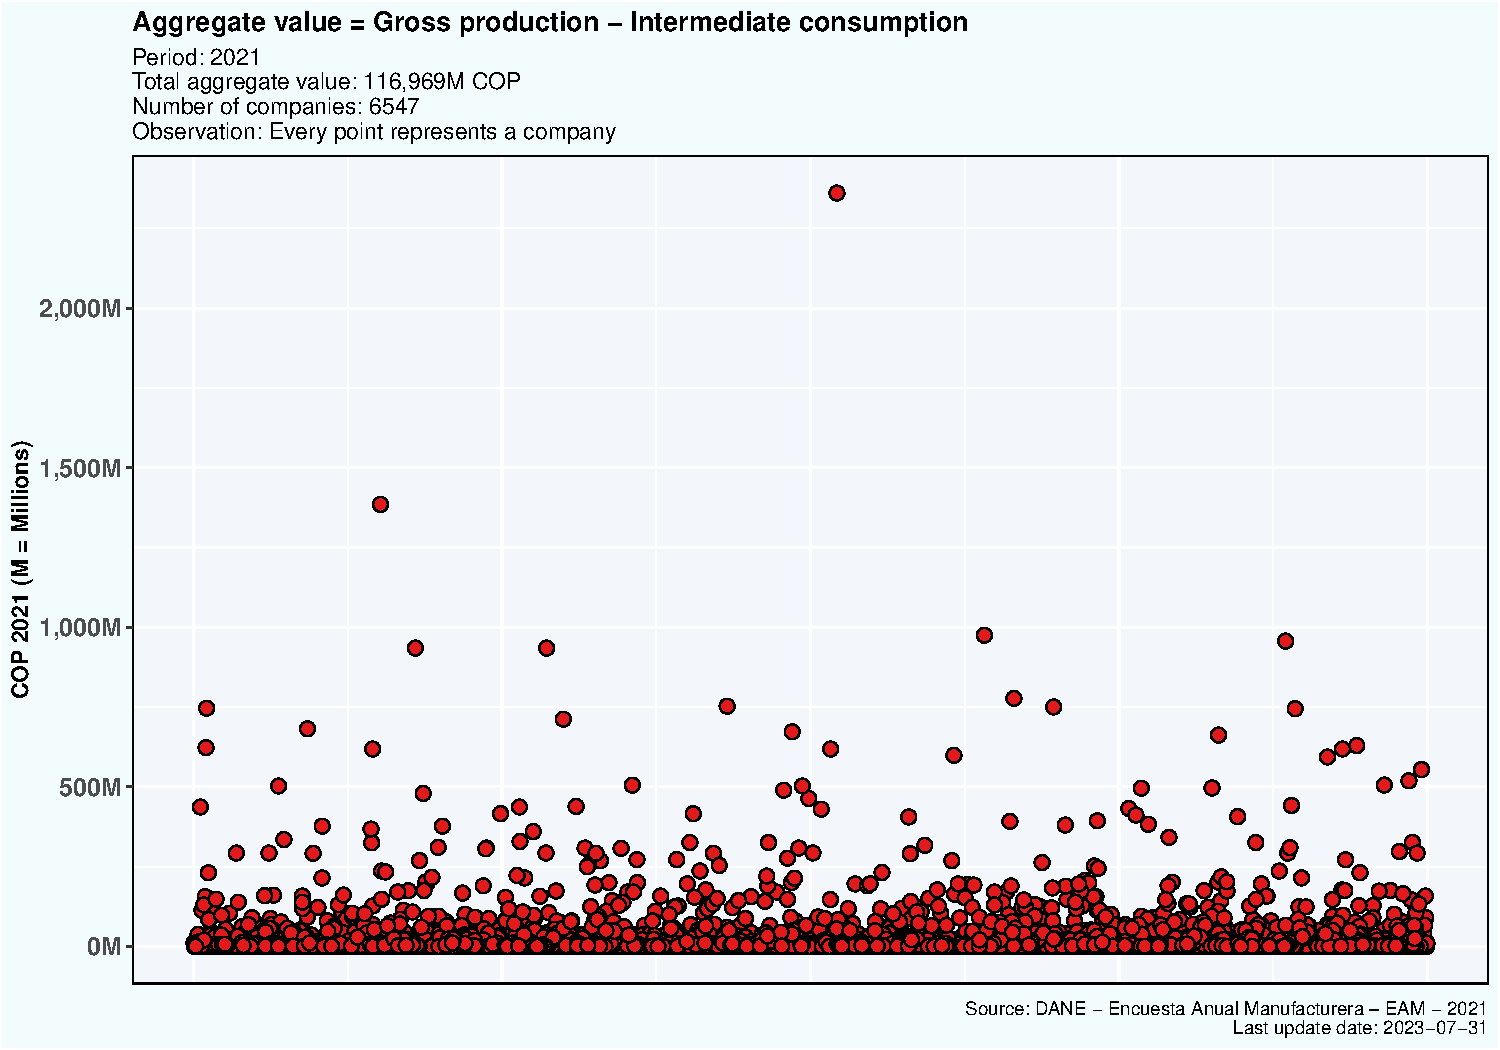
\includegraphics[width=0.85\textwidth,height=\textheight]{001_intro_files/figure-beamer/fig-manufacturing-sector-col-1.pdf}

}

\caption{\label{fig-manufacturing-sector-col}Distribution of aggregate
value in the manufacturing Colombian sector}

\end{figure}%
\end{frame}

\section{Egg wholesale prices}\label{egg-wholesale-prices}

\begin{frame}{}
\phantomsection\label{section-15}
\begin{figure}

\centering{

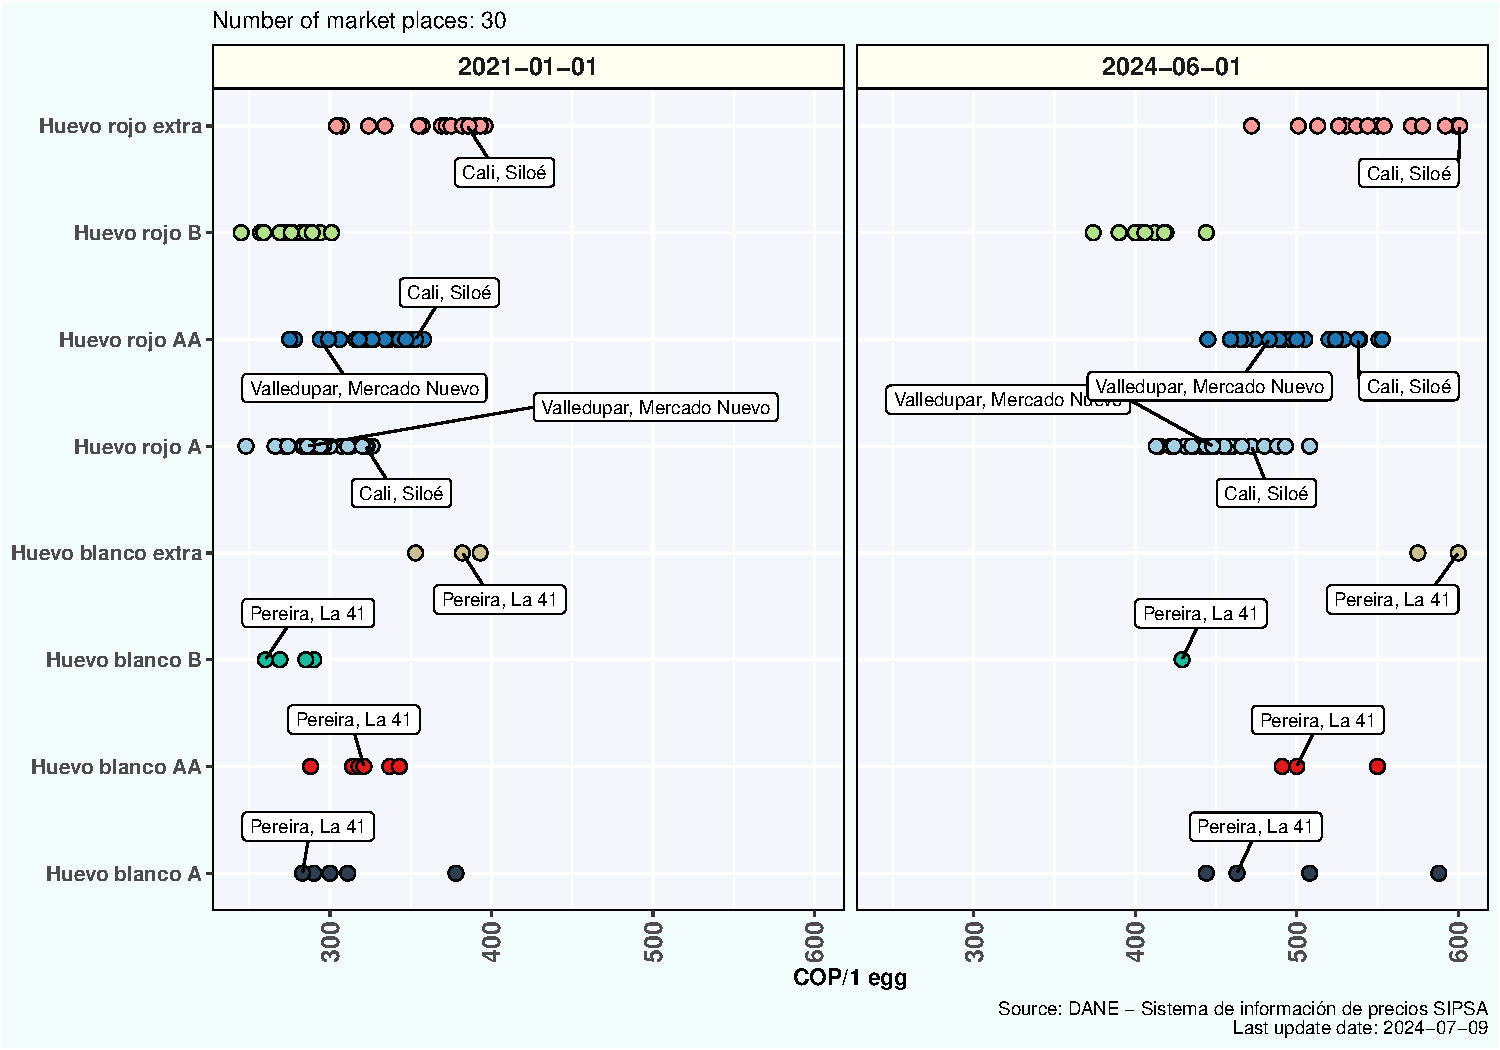
\includegraphics[width=0.85\textwidth,height=\textheight]{001_intro_files/figure-beamer/fig-egg-wholesale-prices-col-1.pdf}

}

\caption{\label{fig-egg-wholesale-prices-col}Egg mean wholesale prices
in Colombian market places}

\end{figure}%
\end{frame}

\section{Flows and stocks}\label{flows-and-stocks}

\begin{frame}{}
\phantomsection\label{section-16}
\begin{itemize}
\item
  \textbf{Stock}: a variable that is measured at a particular point in
  time
\item
  \textbf{Flow}: a variable that is measured over a period of time
\item
  Example \emph{Declaración de Renta Gustavo Francisco Petro Urrego Año
  Gravable 2019}:

  \begin{itemize}
  \item
    \url{https://www.funcionpublica.gov.co/fdci/consultaCiudadana}

    \begin{itemize}
    \tightlist
    \item
      Tipo de persona: NATURAL
    \item
      Primer nombre: Gustavo
    \item
      Segundo nombre: Francisco
    \item
      Primer apellido: Petro
    \item
      Segundo apellido: Urrego
    \end{itemize}
  \end{itemize}
\end{itemize}
\end{frame}

\begin{frame}{}
\phantomsection\label{section-17}
\begin{itemize}
\item
  Patrimonio (stock)

  \begin{itemize}
  \tightlist
  \item
    2019-12-31
  \end{itemize}
\end{itemize}

\begin{center}
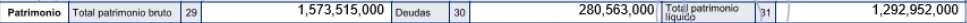
\includegraphics[width=0.6\textwidth,height=\textheight]{000_data/001_patrimonio_petro.png}
\end{center}

\begin{itemize}
\item
  Rentas de trabajo (flow)

  \begin{itemize}
  \tightlist
  \item
    Between 2019-01-01 and 2019-12-31
  \end{itemize}
\end{itemize}

\begin{center}
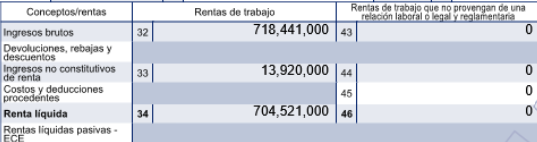
\includegraphics[width=0.6\textwidth,height=\textheight]{000_data/001_rentas_trabajo_petro.png}
\end{center}
\end{frame}

\section{Acknowledgments}\label{acknowledgments}

\begin{frame}{}
\phantomsection\label{section-18}
\begin{itemize}
\item
  To my family that supports me
\item
  To the taxpayers of Colombia and the
  \textbf{\href{https://www.umng.edu.co/estudiante}{UMNG students}} who
  pay my salary
\item
  To the \textbf{\href{https://www.business-science.io/}{Business
  Science}} and \textbf{\href{https://www.rfordatasci.com/}{R4DS Online
  Learning}} communities where I learn
  \textbf{\href{https://www.r-project.org/about.html}{R}} and
  \textbf{\href{https://www.python.org/about/}{\(\pi\)-thon}}
\item
  To the \textbf{\href{https://www.r-project.org/contributors.html}{R
  Core Team}}, the creators of
  \textbf{\href{https://rstudio.com/products/rstudio/}{RStudio IDE}},
  \textbf{\href{https://quarto.org/}{Quarto}} and the authors and
  maintainers of the packages
  \textbf{\href{https://CRAN.R-project.org/package=tidyverse}{tidyverse}},
  \textbf{\href{https://CRAN.R-project.org/package=readxl}{readxl}},
  \textbf{\href{https://CRAN.R-project.org/package=janitor}{janitor}},
  \textbf{\href{https://CRAN.R-project.org/package=scales}{scales}},
  \textbf{\href{https://CRAN.R-project.org/package=knitr}{knitr}},
  \textbf{\href{https://CRAN.R-project.org/package=kableExtra}{kableExtra}},
  \textbf{\href{https://CRAN.R-project.org/package=lubridate}{lubridate}},
  \textbf{\href{https://CRAN.R-project.org/package=ggrepel}{ggrepel}},
  and
  \textbf{\href{https://CRAN.R-project.org/package=tinytex}{tinytex}}
  for allowing me to access these tools without paying for a license
\item
  To the \textbf{\href{https://www.kernel.org/category/about.html}{Linux
  kernel community}} for allowing me the possibility to use some
  \textbf{\href{https://static.lwn.net/Distributions/}{Linux
  distributions}} as my main
  \textbf{\href{https://en.wikipedia.org/wiki/Operating_system}{OS}}
  without paying for a license
\end{itemize}
\end{frame}

\section*{References}\label{references}
\addcontentsline{toc}{section}{References}

\begin{frame}[allowframebreaks]{References}
\phantomsection\label{refs}
\begin{CSLReferences}{1}{0}
\bibitem[\citeproctext]{ref-cardenas_introduccion_2020}
Cardenas, Mauricio. 2020. \emph{Introducción a La {Economía}
{Colombiana}}. 4th ed. Alfaomega.

\bibitem[\citeproctext]{ref-dane_cuestionario_2019}
DANE. 2019. {``Cuestionario {I} {Trimestre} {Etapas} 2001-2002-2003 -
{GEIH} - {Enero} - {Marzo} - 2020.''}
\url{https://microdatos.dane.gov.co/index.php/catalog/780/related-materials}.

\bibitem[\citeproctext]{ref-dane_clasificacion_2022}
---------. 2022a. {``Clasificación {Industrial} {Internacional}
{Uniforme} de Todas Las Actividades Económicas {Revisión} 4 {Adaptada}
Para {Colombia} (2022).''}
\url{https://www.dane.gov.co/files/sen/nomenclatura/ciiu/CIIU_Rev_4_AC2022.pdf}.

\bibitem[\citeproctext]{ref-dane_manual_2022}
---------. 2022b. {``Manual de Recolección y Conceptos y Básicos {GEIH}
{Etapas}: 2210 - 2211 - 2212.''}
\url{https://microdatos.dane.gov.co/index.php/catalog/771/related-materials}.

\bibitem[\citeproctext]{ref-dnp_pobreza_2012}
DNP, and DANE. 2012. {``Pobreza Monetaria En Colombia: Nueva Metodología
y Cifras 2002-2010 Resultados 2ª {Fase} de La {MESEP}.''}
\url{http://microdatos.dane.gov.co/index.php/catalog/708/related_materials}.

\bibitem[\citeproctext]{ref-united_nations_principles_2017}
United Nations. 2017. \emph{Principles and {Recommendations} for
{Population} and {Housing} {Censuses}, {Revision} 3}. Statistical
{Papers} ({Ser}. {M}). UN. \url{https://doi.org/10.18356/bb3ea73e-en}.

\end{CSLReferences}
\end{frame}




\end{document}
